\section{Process Model Description}

\subsection{System Diagram}

The Process Flow Diagram of the system, with all the relevant inputs, outputs and disturbances are displayed in Figure~\ref{fig:PFD}.

\begin{figure}[tbph]
	\centering
	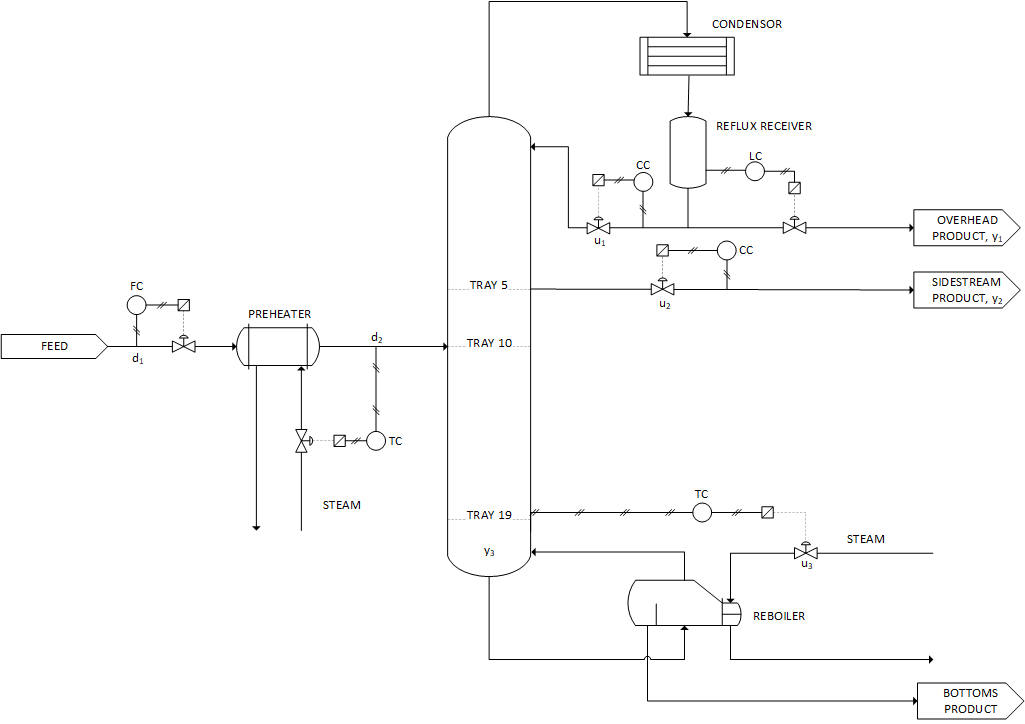
\includegraphics[width=0.9\linewidth]{Figures/Process_PFD}
	\caption{Process flow diagram of the system}
	\label{fig:PFD}
\end{figure}


\subsection{System Description}

The system involves the separation of water and ethanol (in a solution), with the aim of producing an ethanol product that can be used as an alternative fuel source.

The system can be summarized as follows:

\begin{itemize}
	\item The distillation column of the pilot scale plant is a 19 tray, 12 inch diameter column. 
	\item The column has variable feed and side stream draw off locations. 
	\item The side stream flow is varied to control the composition of the stream. 
	\item The distillate vapour draw off stream is fully condensed, and then separated into the reflux and product streams. 
	\item The product stream is set to control the level in the condenser, while the reflux stream controls the composition of the distillate product. 
	\item A kettle re-boiler is used to add energy to the column. Stream is the main utility. 
	\item The amount re-boiled bottoms product is controlled by varying the steam supplied to the re-boiler. 
	\item The feed temperature and flow rate can be controlled to simulate disturbances on the system. These variables are strictly defined as disturbances, as they are part of another section's (the bio-reactor or chemostat) control scheme.
	\item Currently all variables are controlled with single input single output (SISO) control loops.
	
\end{itemize}

\subsection{Measurement of Variables}

The compositions are measured/determined through various on-line sensors (densitrometry and refractometry). Temperatures are monitored using thermocouples. Flow rates are measured with thermal mass flow meters. Levels are measured by inference from static head, measured with a pressure sensor. The product model and serial numbers are not available.


\subsection{System Variables}

All variables in the ethanol water distillation coloumn system is summarised in Table~\ref{tab:Variables}. The current steady state values hold reference to the tested conditions on site.

\begin{table}[H]
	\centering
	\caption{Summary of all the model variables.}
	\begin{tabular}{cccc}
		\hline
		\multicolumn{4}{c}{Input Variables}                                       \\
		
		Variable & Description                       & Steady State Value & Units \\
		\hline
		$u_1$       & Reflux flow rate                  & 0.18               & gpm   \\
		$u_2$       & Side stream product flow rate     & 0.046              & gpm   \\
		$u_3$       & Reboiler steam pressure           & 20                 & psi   \\
		\hline
		\multicolumn{4}{c}{Output Variables}                                      \\
		
		Variable & Description                       & Steady State Value & Units \\
		\hline
		$y_1$       & Overhead ethanol mole fraction    & 0.7                & -     \\
		$y_2$       & Side stream ethanol mole fraction & 0.52               & -     \\
		$y_3$       & Tray \#19 temperature             & 92                 & \si{\celsius} \\
		\hline
		\multicolumn{4}{c}{Disturbance Variables}                                 \\
		
		Variable & Description                       & Steady State Value & Units \\
		\hline
		$d_1$       & Feed flow rate                    & 0.8                & gpm   \\
		$d_2$       & Feed temperature                  & 78                 & \si{\celsius} \\\hline
	\end{tabular}
	\label{tab:Variables}
\end{table}


\subsection{System Model}

The model was determined by conducting pulse testing on the system. In most cases a first order plus dead time model gave a sufficiently accurate fit to experimental data. The sum of squares of an adequate fit during model development was a values of greater than 0.98. In some relationships more complex dynamics had to be derived and a second order system with a first order lag and dead time, was used to accurately describe the impulse response (based on the same adequate fit method described above). The equations used for fitting were

\begin{equation}
	\frac{y_i(s)}{u_i(s)} = \frac{K_i e^{-\theta_is}}{\tau_i s + 1}
\end{equation}

for the first order plus dead time system, and 

\begin{equation}
	\frac{y_i(s)}{u_i(s)} = \frac{K_i (\tau_{1i}s + 1) e ^{-\theta_is +1}}{(\tau_{2i}s +1)(\tau_{3i}s +1)}
\end{equation}

for the relationships with more complex dynamics.

The fitting curves of two pulse tests are displayed in Figure~\ref{fig:test1} and Figure~\ref{fig:test2}. An important thing to note is that the unit of time is minutes, an therefore all responses and analysis will be conducted with this unit for time.

\begin{figure}[htbp]
	\centering
	\begin{minipage}{.48\textwidth}
		\centering
		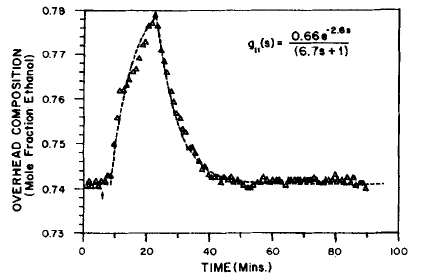
\includegraphics[width=\linewidth]{Figures/Pulse_test_1}
		\captionof{figure}{Overhead composition response to a pulse of 15 minutes duration in the reflux rate.}
		\label{fig:test1}
	\end{minipage}%
	\hfill
	\begin{minipage}{.48\textwidth}
		\centering
		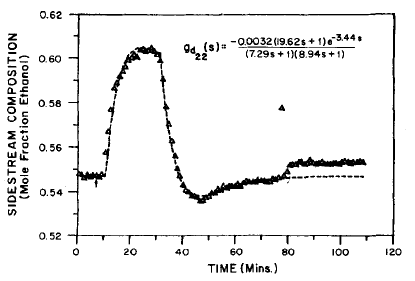
\includegraphics[width=\linewidth]{Figures/Pulse_test_2}
		\captionof{figure}{Side stream composition response to a pulse of 15 minutes duration in feed temperature.}
		\label{fig:test2}
	\end{minipage}
\end{figure}

The model was then written in the standard form of a linear MIMO system \parencite{ogun},

\begin{equation}
\textbf{y}(s) = \textbf{G}(s)\textbf{u}(s) + \textbf{G}_{d}(s)\textbf{d}(s)
\end{equation}

where

\begin{equation}
\hat{G}(s) = \begin{bmatrix}
G_{11} & G_{12} & G_{13} \\
G_{21} & G_{22} & G_{23} \\
G_{31} & G_{32} & G_{33} \\
\end{bmatrix} = \begin{bmatrix}
\frac{0.66e^{-2.6s}}{6.7s+1} & \frac{-0.61e^{-3.5s}}{8.64s+1} & \frac{-0.0049e^{-s}}{9.06s+1} \\
\frac{1.11e^{-6.5s}}{3.25s+1} & \frac{-2.36e^{-3s}}{5.0s+1} & \frac{-0.012e^{-1.2s}}{7.09s+1} \\
\frac{-34.68e^{-9.2s}}{8.15s+1} & \frac{46.2e^{-9.4s}}{10.9s+1} & \frac{0.87(11.61s+1)e^{-s}}{(3.89s+1)(18.8s+1)}
\end{bmatrix}
\end{equation}

and

\begin{equation}
\hat{G_d}(s) = \begin{bmatrix}
G_{d11} & G_{d12} \\
G_{d21} & G_{d22} \\
G_{d31} & G_{d32} \\
\end{bmatrix} = \begin{bmatrix}
\frac{0.14e^{-12s}}{6.2s+1} & \frac{-0.0011(26.32s+1)e^{-2.66s}}{(7.85s+1)(4.63s+1)} \\
\frac{0.53e^{-10.5s}}{6.9s+1} & \frac{-0.0032(19.62s+1)e^{-3.44s}}{(7.29s+1)(8.94s+1)} \\
\frac{-11.54e^{-0.6s}}{7.01s+1} & \frac{0.32e^{-2.6s}}{7.76s+1}
\end{bmatrix}
\end{equation}

\subsection{Scaling the System}
\label{sec:Scaling}
In order to perform a controllability analysis on the system, the system had to be scaled according to the method described in \textcite{skogestad}.

In order to perform the scaling operation, the upper and lower limits of all the variables have to be defined. The initial boundary values of all system variables are summarized in Table~\ref{tab:Manipulated_variables_scaling}, Table~\ref{tab:Controlled_variables_scaling}, and Table~\ref{tab:Disturbance_variables_scaling}.

\begin{table}[H]
	\centering
	\caption{The boundaries of the manipulated variables in the system.}
	\begin{tabular}{cccc}
		\hline
		\textbf{\begin{tabular}[c]{@{}c@{}}Manipulated\\   Variable\end{tabular}} & \textbf{\begin{tabular}[c]{@{}c@{}}Lower \\ Constraint\end{tabular}} & \textbf{\begin{tabular}[c]{@{}c@{}}Upper \\ Constraint\end{tabular}} & \textbf{\begin{tabular}[c]{@{}c@{}}Steady State \\ Value\end{tabular}} \\\hline
		$u_1$, Reflux Flow Rate                                                      & 0.068                                                                & 0.245                                                                & 0.18                                                                   \\
		$u_2$, Side Stream Flow Rate                                                 & 0.00694                                                              & 0.1                                                                  & 0.046                                                                  \\
		$u_3$, Reboiler Steam Pressure                                               & 15.6                                                                 & 34                                                                   & 20                                                                                             
		\\\hline      
	\end{tabular}
	\label{tab:Manipulated_variables_scaling}
\end{table}

\begin{table}[H]
	\centering
	\caption{The boundaries of the controlled variables in the system.}
	\begin{tabular}{ccc}
		\hline
		\textbf{Controlled  Variable}         & \textbf{\begin{tabular}[c]{@{}c@{}}Maximum Set Point \\ Change\end{tabular}} & \textbf{Steady State Value} \\\hline
		$y_1$, Overhead Mole Fraction Ethanol    & 0.05                                                                         & 0.7                         \\
		$y_2$, Side Stream Mole Fraction Ethanol & 0.1                                                                          & 0.52                        \\
		$y_3$, Temperature on Tray \#19          & 8                                                                            & 92                         
		\\\hline      
	\end{tabular}
	\label{tab:Controlled_variables_scaling}
\end{table}

\begin{table}[H]
	\centering
	\caption{The boundaries of the disturbance variables in the system.}
	\begin{tabular}{cccc}
		\hline
		\textbf{\begin{tabular}[c]{@{}c@{}}Disturbance\\   Variable\end{tabular}} & \textbf{\begin{tabular}[c]{@{}c@{}}Lower \\ Constraint\end{tabular}} & \textbf{\begin{tabular}[c]{@{}c@{}}Upper \\ Constraint\end{tabular}} & \textbf{\begin{tabular}[c]{@{}c@{}}Steady State \\ Value\end{tabular}} \\\hline
		d1, Feed Flow Rate            & 0.6                       & 1.1                       & 0.8                         \\
		d2, Feed Temperature          & 50                        & 102                       & 78                         
		\\\hline      
	\end{tabular}
	\label{tab:Disturbance_variables_scaling}
\end{table}

Using the information above the following matrices can be deduced, that will be used to scale the system

\begin{equation}
	D_e = \begin{bmatrix}
	0.01 & 0 & 0 \\
	0 & 0.01 & 0 \\
	0 & 0 & 4 \\
	\end{bmatrix}
\end{equation}

\begin{equation}
D_u = \begin{bmatrix}
0.065 & 0 & 0 \\
0 & 0.03906 & 0 \\
0 & 0 & 4.4 \\
\end{bmatrix}
\end{equation}

\begin{equation}
D_d = \begin{bmatrix}
0.3 & 0 \\
0 & 28 \\
\end{bmatrix}
\end{equation}

\begin{equation}
r = \begin{bmatrix}
0.05 & 0 & 0 \\
0 & 0.1 & 0 \\
0 & 0 & 8 \\
\end{bmatrix}
\end{equation}

Using the above matrices, the scaled system can be calculated using the following equations from [REF!!!],

\begin{equation}
	\label{eq: Scaling 1}
	G = D_e ^{-1}\hat{G}D_u
\end{equation}

\begin{equation}
	\label{eq: Scaling 2}
	G_d = D_e ^{-1}\hat{G_d}D_d
\end{equation}

From Equation~\ref{eq: Scaling 1} and Equation~\ref{eq: Scaling 2}, the scaled system can be written as 

\begin{equation}
G(s) = \begin{bmatrix}
G_{11} & G_{12} & G_{13} \\
G_{21} & G_{22} & G_{23} \\
G_{31} & G_{32} & G_{33} \\
\end{bmatrix} = \begin{bmatrix}
\frac{4.29e^{-2.6s}}{6.7s+1} & \frac{-2.38266e^{-3.5s}}{8.64s+1} & \frac{-2.156e^{-s}}{9.06s+1} \\
\frac{7.215e^{-6.5s}}{3.25s+1} & \frac{-9.21816e^{-3s}}{5.0s+1} & \frac{-2.156e^{-1.2s}}{7.09s+1} \\
\frac{-0.56355e^{-9.2s}}{8.15s+1} & \frac{0.451143e^{-9.4s}}{10.9s+1} & \frac{1.1(10.1007s+0.87)e^{-s}}{(3.89s+1)(18.8s+1)}
\end{bmatrix}
\end{equation}

and

\begin{equation}
G_d(s) = \begin{bmatrix}
G_{d11} & G_{d12} \\
G_{d21} & G_{d22} \\
G_{d31} & G_{d32} \\
\end{bmatrix} = \begin{bmatrix}
\frac{4.2e^{-12s}}{6.2s+1} & \frac{-2800(0.028952s+0.0011)e^{-2.66s}}{(7.85s+1)(4.63s+1)} \\
\frac{15.9e^{-10.5s}}{6.9s+1} & \frac{-2800(-0.062784s+0.0032)e^{-3.44s}}{(7.29s+1)(8.94s+1)} \\
\frac{-0.8655e^{-0.6s}}{7.01s+1} & \frac{2.24e^{-2.6s}}{7.76s+1}
\end{bmatrix}
\end{equation}

with 

\begin{equation}
R = \begin{bmatrix}
5 & 0 & 0 \\
0 & 10 & 0 \\
0 & 0 & 2 \\
\end{bmatrix}
\end{equation}